% Created 2022-08-23 ter 22:27
% Intended LaTeX compiler: pdflatex
\documentclass[t, aspectratio=169]{beamer}
\usepackage[utf8]{inputenc}
\usepackage[T1]{fontenc}
\usepackage{graphicx}
\usepackage{longtable}
\usepackage{wrapfig}
\usepackage{rotating}
\usepackage[normalem]{ulem}
\usepackage{amsmath}
\usepackage{amssymb}
\usepackage{capt-of}
\usepackage{hyperref}
\usepackage[newfloat]{minted}
\usepackage{tikz}
\usetheme{default}
\author{Luigi D. C. Soares}
\date{DCC/UFMG (25/08/2022)}
\title{Linguagem C - Introdução}
\subtitle{Progamação e Desenvolvimento de Software I}
\title[Linguagem C]{Linguagem C - Introdução}
\subtitle{Programação e Desenvolvimento de Software I}
\author[\tiny\{gleison.mendonca, luigi.domenico\}@dcc.ufmg.br]{%
Gleison S. D. Mendonça, Luigi D. C. Soares\texorpdfstring{\\}{}
\texttt{\{gleison.mendonca, luigi.domenico\}@dcc.ufmg.br}}
\institute[DCC/UFMG]{}
\date[25/08/2022]{}
%\usetheme{saori}
%\usemintedstyle{native}
\usetheme{ufmg}
\hypersetup{
 pdfauthor={Luigi D. C. Soares},
 pdftitle={Linguagem C - Introdução},
 pdfkeywords={},
 pdfsubject={},
 pdfcreator={Emacs 28.1 (Org mode 9.6)}, 
 pdflang={English}}
\begin{document}

\maketitle

\begin{frame}[label={sec:org3273e32}]{Linguagem C}
\begin{itemize}
\item Criada em 1972

\item Linguagem imperativa
\begin{itemize}
\item Uso de comandos: Se \alert{x} \uline{Faça!} \alert{y}
\item Comandos alteram o estado do programa
\end{itemize}
\end{itemize}
\end{frame}

\begin{frame}[label={sec:org6c7ed8f}]{Linguagem C}
\begin{itemize}
\item Criada em 1972

\item Linguagem imperativa
\begin{itemize}
\item Uso de comandos: Se \alert{x} \uline{Faça!} \alert{y}
\item Comandos alteram o estado do programa
\end{itemize}

\item Linguagem procedural
\begin{itemize}
\item Decomposição de um problema em diferentes funções e módulos
\item Reutilização de código
\end{itemize}
\end{itemize}
\end{frame}

\begin{frame}[label={sec:org9172e06}]{Linguagem C}
\begin{itemize}
\item Criada em 1972

\item Linguagem imperativa
\begin{itemize}
\item Uso de comandos: Se \alert{x} \uline{Faça!} \alert{y}
\item Comandos alteram o estado do programa
\end{itemize}

\item Linguagem procedural
\begin{itemize}
\item Decomposição de um problema em diferentes funções e módulos
\item Reutilização de código
\end{itemize}

\item Acesso de baixo nível á memória
\item Utilização de instruções Assembly (código de máquina)
\item Gera códigos geralmente mais velozes
\end{itemize}
\end{frame}

\begin{frame}[label={sec:org2cbc23e}]{Linguagem C}
\begin{itemize}
\item Criada em 1972

\item Linguagem imperativa
\begin{itemize}
\item Uso de comandos: Se \alert{x} \uline{Faça!} \alert{y}
\item Comandos alteram o estado do programa
\end{itemize}

\item Linguagem procedural
\begin{itemize}
\item Decomposição de um problema em diferentes funções e módulos
\item Reutilização de código
\end{itemize}

\item Acesso de baixo nível á memória
\item Utilização de instruções Assembly (código de máquina)
\item Gera códigos geralmente mais velozes

\item Sair de C para outras linguagens é mais fácil que o sentido oposto
\end{itemize}
\end{frame}

\begin{frame}[label={sec:orgcdd8b45},fragile]{Primeiro programa em C}
 \begin{minted}[,frame=lines,framesep=2mm,linenos]{c}
#include <stdio.h> // Inclusão do módulo de entrada/saída

// Ponto de entrada do programa
int main(int argc, char *argv[]) {
    // TODO
    return 0;
}
\end{minted}
\end{frame}

\begin{frame}[label={sec:orgf98fe18},fragile]{Primeiro programa em C}
 \begin{minted}[,frame=lines,framesep=2mm,linenos]{c}
#include <stdio.h> // Inclusão do módulo de entrada/saída

// Ponto de entrada do programa
int main(int argc, char *argv[]) {
    // Escreve uma mensagem na tela de saída
    printf("Olá mundo\n");
    return 0;
}
\end{minted}
\end{frame}

\begin{frame}[label={sec:org7b79493}]{Indentação}
\begin{itemize}
\item Espaçamento colocado antes de começar a escrever o código na linha
\end{itemize}
\end{frame}

\begin{frame}[label={sec:org0afce78},fragile]{Indentação}
 \begin{itemize}
\item Espaçamento colocado antes de começar a escrever o código na linha
\item É importante!
\end{itemize}

\begin{minted}[,frame=lines,framesep=2mm,linenos]{c}
#include <stdio.h>
int main(int argc, char *argv[]) { printf("Olá mundo\n"); return 0; }
\end{minted}
\end{frame}

\begin{frame}[label={sec:orgd7758e3}]{Primeiro problema}
Suponha que soma (+) e subtração (-) são as únicas operações disponíveis.

Dados dois números inteiros positivos \alert{A} e \alert{B}, determine o \alert{quociente} e o \alert{resto}
da divisão de \alert{A} por \alert{B.}
\end{frame}

\begin{frame}[label={sec:org58877e9}]{Primeiro problema}
\alert{Ideia de solução}:
\begin{itemize}
\item Representar os números \alert{A} e \alert{B} por retângulos de \alert{larguras} proporcionais aos seus valores
\item Verificar quantas vezes \alert{B} cabe em \alert{A}
\end{itemize}
\vspace{0.5em}\centering\tikzset{every picture/.style={line width=0.75pt}} %set default line width to 0.75pt
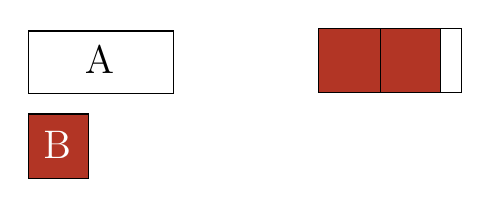
\begin{tikzpicture}[x=0.75pt,y=0.75pt,yscale=-1,xscale=1]
%uncomment if require: \path (0,126); %set diagram left start at 0, and has height of 126

%Shape: Rectangle [id:dp7852098459874652]
\draw  [fill={rgb, 255:red, 255; green, 255; blue, 255 }  ,fill opacity=1 ] (41,21) -- (111,21) -- (111,51.03) -- (41,51.03) -- cycle ;
%Shape: Rectangle [id:dp35920484998714075]
\draw  [fill={rgb, 255:red, 178; green, 53; blue, 37 }  ,fill opacity=1 ] (41,61) -- (70.01,61) -- (70.01,92.03) -- (41,92.03) -- cycle ;
%Shape: Rectangle [id:dp31032605623178733]
\draw  [fill={rgb, 255:red, 178; green, 53; blue, 37 }  ,fill opacity=1 ] (180.67,19.67) -- (210.68,19.67) -- (210.68,50.7) -- (180.67,50.7) -- cycle ;
%Shape: Rectangle [id:dp9954521977784945]
\draw  [fill={rgb, 255:red, 178; green, 53; blue, 37 }  ,fill opacity=1 ] (210.68,19.67) -- (239.69,19.67) -- (239.69,50.7) -- (210.68,50.7) -- cycle ;
%Shape: Rectangle [id:dp0077618542939301705]
\draw  [fill={rgb, 255:red, 255; green, 255; blue, 255 }  ,fill opacity=1 ] (239.69,19.67) -- (249.67,19.67) -- (249.67,50.7) -- (239.69,50.7) -- cycle ;

% Text Node
\draw (67,27) node [anchor=north west][inner sep=0.75pt]  [font=\Large,color={rgb, 255:red, 0; green, 0; blue, 0 }  ,opacity=1 ] [align=left] {A};
% Text Node
\draw (47,68) node [anchor=north west][inner sep=0.75pt]  [font=\Large,color={rgb, 255:red, 255; green, 255; blue, 255 }  ,opacity=1 ] [align=left] {B};
\end{tikzpicture}

\begin{itemize}
\item \alert{A = 7}
\item \alert{B = 3}
\end{itemize}
\end{frame}

\begin{frame}[label={sec:orgc198678}]{Algoritmo}
\begin{itemize}
\item Para resolver um problema, primeiro precisamos de uma descrição clara da solução
\item Um algoritmo é uma sequência de instruções (receita)
\begin{itemize}
\item Finita
\item Não pode ser ambígua
\end{itemize}
\end{itemize}
\end{frame}

\begin{frame}[label={sec:org014e9fa}]{Algoritmo}
\begin{itemize}
\item Para resolver um problema, primeiro precisamos de uma descrição clara da solução
\item Um algoritmo é uma sequência de instruções (receita)
\begin{itemize}
\item Finita
\item Não pode ser ambígua
\end{itemize}
\end{itemize}

\alert{Voltando ao nosso problema:}
\end{frame}

\begin{frame}[label={sec:org5f8261a}]{Algoritmo}
\begin{itemize}
\item Para resolver um problema, primeiro precisamos de uma descrição clara da solução
\item Um algoritmo é uma sequência de instruções (receita)
\begin{itemize}
\item Finita
\item Não pode ser ambígua
\end{itemize}
\end{itemize}

\alert{Voltando ao nosso problema:}

\begin{itemize}
\item Sejam A e B os valores dados
\item Atribuir o valor 0 ao quociente (q)
\end{itemize}
\end{frame}

\begin{frame}[label={sec:org1b2b626}]{Algoritmo}
\begin{itemize}
\item Para resolver um problema, primeiro precisamos de uma descrição clara da solução
\item Um algoritmo é uma sequência de instruções (receita)
\begin{itemize}
\item Finita
\item Não pode ser ambígua
\end{itemize}
\end{itemize}

\alert{Voltando ao nosso problema:}

\begin{itemize}
\item Sejam A e B os valores dados
\item Atribuir o valor 0 ao quociente (q)
\item Enquanto \alert{B <= A}:
\end{itemize}
\end{frame}

\begin{frame}[label={sec:orgaa9a71d}]{Algoritmo}
\begin{itemize}
\item Para resolver um problema, primeiro precisamos de uma descrição clara da solução
\item Um algoritmo é uma sequência de instruções (receita)
\begin{itemize}
\item Finita
\item Não pode ser ambígua
\end{itemize}
\end{itemize}

\alert{Voltando ao nosso problema:}

\begin{itemize}
\item Sejam A e B os valores dados
\item Atribuir o valor 0 ao quociente (q)
\item Enquanto \alert{B <= A}:
\begin{itemize}
\item Somar 1 ao valor de q
\item Subtrair B do valor de A
\end{itemize}
\end{itemize}
\end{frame}

\begin{frame}[label={sec:orga0dbc4e}]{Algoritmo}
\begin{itemize}
\item Para resolver um problema, primeiro precisamos de uma descrição clara da solução
\item Um algoritmo é uma sequência de instruções (receita)
\begin{itemize}
\item Finita
\item Não pode ser ambígua
\end{itemize}
\end{itemize}

\alert{Voltando ao nosso problema:}

\begin{itemize}
\item Sejam A e B os valores dados
\item Atribuir o valor 0 ao quociente (q)
\item Enquanto \alert{B <= A}:
\begin{itemize}
\item Somar 1 ao valor de q
\item Subtrair B do valor de A
\end{itemize}
\item Atribuir o valor final de A ao resto (r)
\end{itemize}
\end{frame}

\begin{frame}[label={sec:org8ee3060},fragile]{Implementando o algoritmo}
 \vspace{-2em}
\begin{minted}[,frame=lines,framesep=2mm,linenos]{c}
#include <stdio.h>
int main(int argc, char *argv[]) {
    // TODO
}
\end{minted}
\end{frame}

\begin{frame}[label={sec:orgfd0cadc},fragile]{Implementando o algoritmo}
 \vspace{-2em}
\begin{minted}[,frame=lines,framesep=2mm,linenos]{c}
#include <stdio.h>
int main(int argc, char *argv[]) {
    int a = 7;
    int b = 3;
    int q = 0; // Inicializando quociente
    while (b <= a) {
        q = q + 1; // Somar 1 ao valor de q
        a = a - b; // Subtrair B do valor de A
    }
    int r = a; // resto = valor final de A
    printf("Quociente: %d\n", q);
    printf("Resto:  %d\n", r);
    return 0;
}
\end{minted}
\end{frame}

\begin{frame}[label={sec:orgf6fca31}]{Algoritmo vs Implementação}
\begin{itemize}
\item Note que o algoritmo (pseudo-código) que escrevemos anteriormente é mais
flexível, sem muitas regras
\item A implementação em alguma linguagem (nosso caso = C), por outro lado, obedece
\alert{regras de sintaxe}
\end{itemize}
\end{frame}

\begin{frame}[label={sec:org8273691}]{Erro de Sintaxe}
\begin{itemize}
\item Em C, todo comando deve ser terminado por ponto e vírgula
\end{itemize}
\end{frame}

\begin{frame}[label={sec:orgcc6749b},fragile]{Erro de Sintaxe}
 \begin{itemize}
\item Em C, todo comando deve ser terminado por ponto e vírgula
\end{itemize}

\begin{minted}[,frame=lines,framesep=2mm,linenos]{c}
#include <stdio.h>
int main(int argc, char *argv[]) {
    int a = 7;
    return 0 // expected ';' before '}' token
}
\end{minted}
\end{frame}

\begin{frame}[label={sec:org90965ab},fragile]{Erro de Lógica}
 \begin{itemize}
\item \alert{Atenção!} Não basta obter um programa executável!! Será que ele está correto?
\item Considere o seguinte problema: determinar e exibir o valor de \texttt{y = seno(1,5)}
\end{itemize}
\begin{minted}[,frame=lines,framesep=2mm,linenos]{c}
#include <stdio.h>
#include <math.h>

int main(int argc, char *argv[]) {
    // TODO
    return 0;
}
\end{minted}
\end{frame}

\begin{frame}[label={sec:orgce01039},fragile]{Erro de Lógica}
 \begin{itemize}
\item \alert{Atenção!} Não basta obter um programa executável!! Será que ele está correto?
\item Considere o seguinte problema: determinar e exibir o valor de \texttt{y = seno(1,5)}
\end{itemize}
\begin{minted}[,frame=lines,framesep=2mm,linenos]{c}
#include <stdio.h>
#include <math.h>

int main(int argc, char *argv[]) {
    float y = sin(1.5);
    printf("seno de 1,5 = %f\n", y);
    return 0;
}
\end{minted}
\end{frame}

\begin{frame}[label={sec:org05951be},fragile]{Erro de Lógica}
 \begin{itemize}
\item Se ao invés de \texttt{y = sin(1.5);} tivéssemos escrito \texttt{y = sin(2.5)}, o programa seria produzido e executaria normalmente
\end{itemize}
\begin{minted}[,frame=lines,framesep=2mm,linenos]{c}
#include <stdio.h>
#include <math.h>

int main(int argc, char *argv[]) {
    float y = sin(2.5);
    printf("seno de 1,5 = %f\n", y);
    return 0;
}
\end{minted}
\end{frame}

\begin{frame}[label={sec:org8f2d83d},fragile]{Erro de Lógica}
 \begin{itemize}
\item Se ao invés de \texttt{y = sin(1.5);} tivéssemos escrito \texttt{y = sin(2.5)}, o programa seria produzido e executaria normalmente
\item Embora um resultado tenha sido obtido, ele \alert{não é correto}
\item Se um programa executável não produz os resultados corretos, é porque ele contém \alert{erros de lógica} ou \alert{bugs}
\item O processo de identificação e correção de erros de lógica é denominado \alert{depuração} (\alert{debug}).
\end{itemize}
\end{frame}

\begin{frame}[label={sec:org74c1e94}]{Como o computador entende o que escrevemos?}
\begin{itemize}
\item Nosso programa em C é um texto
\item O computador entende textos?
\end{itemize}
\end{frame}

\begin{frame}[label={sec:org04961d4}]{Como o computador entende o que escrevemos?}
\begin{itemize}
\item Nosso programa em C é um texto
\item O computador entende textos?
\item \alert{Não!} Computadores executam instruções escritas em formato binário (0's e 1's)
\item Precisamos traduzir nosso texto para \alert{linguagem de máquina}
\end{itemize}
\end{frame}

\begin{frame}[label={sec:org3ff4305}]{Como o computador entende o que escrevemos?}
\begin{itemize}
\item Nosso programa em C é um texto
\item O computador entende textos?
\item \alert{Não!} Computadores executam instruções escritas em formato binário (0's e 1's)
\item Precisamos traduzir nosso texto para \alert{linguagem de máquina}
\end{itemize}

\centering\vspace{0.5em}\tikzset{every picture/.style={line width=0.75pt}} %set default line width to 0.75pt
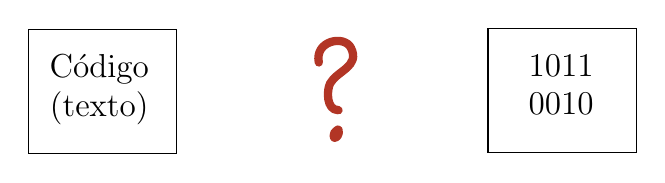
\begin{tikzpicture}[x=0.75pt,y=0.75pt,yscale=-1,xscale=1]
%uncomment if require: \path (0,170); %set diagram left start at 0, and has height of 170

%Shape: Rectangle [id:dp7852098459874652]
\draw  [fill={rgb, 255:red, 255; green, 255; blue, 255 }  ,fill opacity=1 ] (99,50) -- (170.5,50) -- (170.5,110) -- (99,110) -- cycle ;
%Shape: Rectangle [id:dp240405123901279]
\draw  [fill={rgb, 255:red, 255; green, 255; blue, 255 }  ,fill opacity=1 ] (320.5,49.5) -- (392,49.5) -- (392,109.5) -- (320.5,109.5) -- cycle ;
%Shape: Free Drawing [id:dp02650560539042357]
\draw  [color={rgb, 255:red, 178; green, 53; blue, 37 }  ,draw opacity=1 ][line width=3] [line join = round][line cap = round] (239,66) .. controls (236.9,55.48) and (251.28,52.56) .. (254.5,59) .. controls (258.98,67.97) and (247.87,69.94) .. (244.5,76) .. controls (242.78,79.1) and (242.41,89) .. (248.5,89) ;
%Shape: Free Drawing [id:dp11935749666588036]
\draw  [color={rgb, 255:red, 178; green, 53; blue, 37 }  ,draw opacity=1 ][line width=3] [line join = round][line cap = round] (247,100) .. controls (247,96.96) and (244.7,104.8) .. (248,101.5) .. controls (248.72,100.78) and (248.67,99.5) .. (248.5,98.5) .. controls (248.34,97.56) and (246.71,100) .. (246.5,100) ;

% Text Node
\draw (102,61) node [anchor=north west][inner sep=0.75pt]  [font=\large,color={rgb, 255:red, 0; green, 0; blue, 0 }  ,opacity=1 ] [align=left] {\begin{minipage}[lt]{44.91pt}\setlength\topsep{0pt}
\begin{center}
Código \\(texto)
\end{center}

\end{minipage}};
% Text Node
\draw (330,61) node [anchor=north west][inner sep=0.75pt]  [font=\large,color={rgb, 255:red, 0; green, 0; blue, 0 }  ,opacity=1 ] [align=left] {\begin{minipage}[lt]{36.76pt}\setlength\topsep{0pt}
\begin{center}
1011\\0010
\end{center}

\end{minipage}};

\end{tikzpicture}
\end{frame}

\begin{frame}[label={sec:orgdab7166}]{Como o computador entende o que escrevemos?}
\begin{itemize}
\item Nosso programa em C é um texto
\item O computador entende textos?
\item \alert{Não!} Computadores executam instruções escritas em formato binário (0's e 1's)
\item Precisamos traduzir nosso texto para \alert{linguagem de máquina}
\end{itemize}

\centering\vspace{0.5em}\tikzset{every picture/.style={line width=0.75pt}} %set default line width to 0.75pt
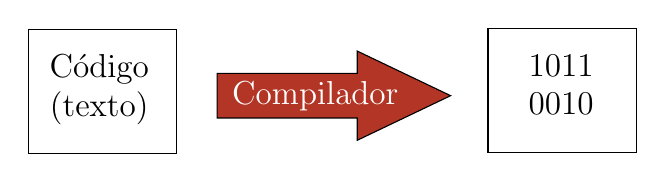
\begin{tikzpicture}[x=0.75pt,y=0.75pt,yscale=-1,xscale=1]
%uncomment if require: \path (0,170); %set diagram left start at 0, and has height of 170

%Shape: Rectangle [id:dp7852098459874652]
\draw  [fill={rgb, 255:red, 255; green, 255; blue, 255 }  ,fill opacity=1 ] (99,50) -- (170.5,50) -- (170.5,110) -- (99,110) -- cycle ;
%Shape: Rectangle [id:dp240405123901279]
\draw  [fill={rgb, 255:red, 255; green, 255; blue, 255 }  ,fill opacity=1 ] (320.5,49.5) -- (392,49.5) -- (392,109.5) -- (320.5,109.5) -- cycle ;
%Right Arrow [id:dp6605035354622533]
\draw  [fill={rgb, 255:red, 178; green, 53; blue, 37 }  ,fill opacity=1 ] (190,71.25) -- (257.5,71.25) -- (257.5,60.5) -- (302.5,82) -- (257.5,103.5) -- (257.5,92.75) -- (190,92.75) -- cycle ;

% Text Node
\draw (102,61) node [anchor=north west][inner sep=0.75pt]  [font=\large,color={rgb, 255:red, 0; green, 0; blue, 0 }  ,opacity=1 ] [align=left] {\begin{minipage}[lt]{44.91pt}\setlength\topsep{0pt}
\begin{center}
Código \\(texto)
\end{center}

\end{minipage}};
% Text Node
\draw (330,61) node [anchor=north west][inner sep=0.75pt]  [font=\large,color={rgb, 255:red, 0; green, 0; blue, 0 }  ,opacity=1 ] [align=left] {\begin{minipage}[lt]{36.76pt}\setlength\topsep{0pt}
\begin{center}
1011\\0010
\end{center}

\end{minipage}};
% Text Node
\draw (192.5,74) node [anchor=north west][inner sep=0.75pt]  [font=\large,color={rgb, 255:red, 255; green, 255; blue, 255 }  ,opacity=1 ] [align=left] {\begin{minipage}[lt]{65.31pt}\setlength\topsep{0pt}
\begin{center}
Compilador
\end{center}

\end{minipage}};

\end{tikzpicture}
\end{frame}

\begin{frame}[label={sec:orgc219f94},fragile]{Como o computador entende o que escrevemos?}
 \begin{itemize}
\item Nosso programa em C é um texto
\item O computador entende textos?
\item \alert{Não!} Computadores executam instruções escritas em formato binário (0's e 1's)
\item Precisamos traduzir nosso texto para \alert{linguagem de máquina}
\end{itemize}

\centering\vspace{0.5em}\tikzset{every picture/.style={line width=0.75pt}} %set default line width to 0.75pt
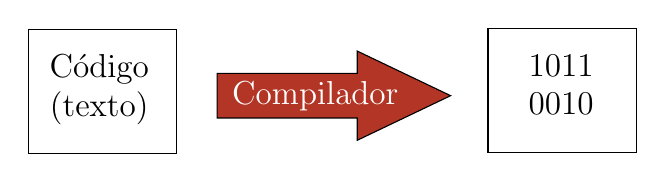
\begin{tikzpicture}[x=0.75pt,y=0.75pt,yscale=-1,xscale=1]
%uncomment if require: \path (0,170); %set diagram left start at 0, and has height of 170

%Shape: Rectangle [id:dp7852098459874652]
\draw  [fill={rgb, 255:red, 255; green, 255; blue, 255 }  ,fill opacity=1 ] (99,50) -- (170.5,50) -- (170.5,110) -- (99,110) -- cycle ;
%Shape: Rectangle [id:dp240405123901279]
\draw  [fill={rgb, 255:red, 255; green, 255; blue, 255 }  ,fill opacity=1 ] (320.5,49.5) -- (392,49.5) -- (392,109.5) -- (320.5,109.5) -- cycle ;
%Right Arrow [id:dp6605035354622533]
\draw  [fill={rgb, 255:red, 178; green, 53; blue, 37 }  ,fill opacity=1 ] (190,71.25) -- (257.5,71.25) -- (257.5,60.5) -- (302.5,82) -- (257.5,103.5) -- (257.5,92.75) -- (190,92.75) -- cycle ;

% Text Node
\draw (102,61) node [anchor=north west][inner sep=0.75pt]  [font=\large,color={rgb, 255:red, 0; green, 0; blue, 0 }  ,opacity=1 ] [align=left] {\begin{minipage}[lt]{44.91pt}\setlength\topsep{0pt}
\begin{center}
Código \\(texto)
\end{center}

\end{minipage}};
% Text Node
\draw (330,61) node [anchor=north west][inner sep=0.75pt]  [font=\large,color={rgb, 255:red, 0; green, 0; blue, 0 }  ,opacity=1 ] [align=left] {\begin{minipage}[lt]{36.76pt}\setlength\topsep{0pt}
\begin{center}
1011\\0010
\end{center}

\end{minipage}};
% Text Node
\draw (192.5,74) node [anchor=north west][inner sep=0.75pt]  [font=\large,color={rgb, 255:red, 255; green, 255; blue, 255 }  ,opacity=1 ] [align=left] {\begin{minipage}[lt]{65.31pt}\setlength\topsep{0pt}
\begin{center}
Compilador
\end{center}

\end{minipage}};

\end{tikzpicture}

\begin{itemize}
\item O processo de ``tradução'' do código é chamado de \alert{compilação}
\item O \alert{compilador} recebe o \alert{código fonte} e produz um \alert{programa executável}
\item \texttt{gcc main.c -o main}
\end{itemize}
\end{frame}

\begin{frame}[label={sec:orgb729d65}]{Compilação}
\begin{itemize}
\item É um pouquinho mais complexo que isso
\end{itemize}
\end{frame}

\begin{frame}[label={sec:org3d15f06}]{Compilação}
\begin{itemize}
\item É um pouquinho mais complexo que isso
\end{itemize}

\centering\vspace{0.5em}\tikzset{every picture/.style={line width=0.75pt}} %set default line width to 0.75pt
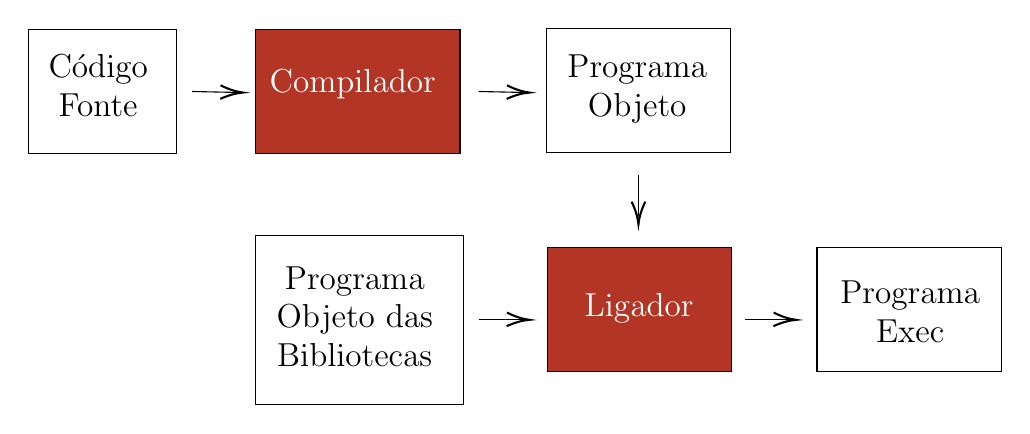
\begin{tikzpicture}[x=0.75pt,y=0.75pt,yscale=-1,xscale=1]
%uncomment if require: \path (0,270); %set diagram left start at 0, and has height of 270

%Shape: Rectangle [id:dp7852098459874652]
\draw  [fill={rgb, 255:red, 255; green, 255; blue, 255 }  ,fill opacity=1 ] (11,50) -- (82.5,50) -- (82.5,110) -- (11,110) -- cycle ;
%Shape: Rectangle [id:dp240405123901279]
\draw  [fill={rgb, 255:red, 255; green, 255; blue, 255 }  ,fill opacity=1 ] (260.5,49.5) -- (349.5,49.5) -- (349.5,109.5) -- (260.5,109.5) -- cycle ;
%Straight Lines [id:da08666006294713702]
\draw    (90,79.98) -- (112.5,80.46) ;
\draw [shift={(114.5,80.5)}, rotate = 181.21] [color={rgb, 255:red, 0; green, 0; blue, 0 }  ][line width=0.75]    (10.93,-3.29) .. controls (6.95,-1.4) and (3.31,-0.3) .. (0,0) .. controls (3.31,0.3) and (6.95,1.4) .. (10.93,3.29)   ;
%Shape: Rectangle [id:dp38842710070627606]
\draw  [fill={rgb, 255:red, 178; green, 53; blue, 37 }  ,fill opacity=1 ] (120.5,50) -- (219,50) -- (219,110) -- (120.5,110) -- cycle ;
%Straight Lines [id:da5494063713073924]
\draw    (228,79.98) -- (250.5,80.46) ;
\draw [shift={(252.5,80.5)}, rotate = 181.21] [color={rgb, 255:red, 0; green, 0; blue, 0 }  ][line width=0.75]    (10.93,-3.29) .. controls (6.95,-1.4) and (3.31,-0.3) .. (0,0) .. controls (3.31,0.3) and (6.95,1.4) .. (10.93,3.29)   ;
%Shape: Rectangle [id:dp10236773740516991]
\draw  [fill={rgb, 255:red, 178; green, 53; blue, 37 }  ,fill opacity=1 ] (261,155) -- (350,155) -- (350,215) -- (261,215) -- cycle ;
%Straight Lines [id:da28904142100608676]
\draw    (305,120) -- (305,140) ;
\draw [shift={(305,144)}, rotate = 270] [color={rgb, 255:red, 0; green, 0; blue, 0 }  ][line width=0.75]    (10.93,-3.29) .. controls (6.95,-1.4) and (3.31,-0.3) .. (0,0) .. controls (3.31,0.3) and (6.95,1.4) .. (10.93,3.29)   ;
%Shape: Rectangle [id:dp312816305480381]
\draw  [fill={rgb, 255:red, 255; green, 255; blue, 255 }  ,fill opacity=1 ] (120.5,149.5) -- (220.5,149.5) -- (220.5,231) -- (120.5,231) -- cycle ;
%Straight Lines [id:da17984903366089666]
\draw    (228,190) -- (250.5,190) ;
\draw [shift={(252.5,190)}, rotate = 181.21] [color={rgb, 255:red, 0; green, 0; blue, 0 }  ][line width=0.75]    (10.93,-3.29) .. controls (6.95,-1.4) and (3.31,-0.3) .. (0,0) .. controls (3.31,0.3) and (6.95,1.4) .. (10.93,3.29)   ;
%Shape: Rectangle [id:dp9233001220236068]
\draw  [fill={rgb, 255:red, 255; green, 255; blue, 255 }  ,fill opacity=1 ] (391,155) -- (480,155) -- (480,215) -- (391,215) -- cycle ;
%Straight Lines [id:da8370387235079737]
\draw    (356.5,190) -- (379,190) ;
\draw [shift={(381,190)}, rotate = 181.21] [color={rgb, 255:red, 0; green, 0; blue, 0 }  ][line width=0.75]    (10.93,-3.29) .. controls (6.95,-1.4) and (3.31,-0.3) .. (0,0) .. controls (3.31,0.3) and (6.95,1.4) .. (10.93,3.29)   ;

% Text Node
\draw (13.5,61) node [anchor=north west][inner sep=0.75pt]  [font=\large,color={rgb, 255:red, 0; green, 0; blue, 0 }  ,opacity=1 ] [align=left] {\begin{minipage}[lt]{44.91pt}\setlength\topsep{0pt}
\begin{center}
Código \\Fonte
\end{center}

\end{minipage}};
% Text Node
\draw (265.5,61) node [anchor=north west][inner sep=0.75pt]  [font=\large,color={rgb, 255:red, 0; green, 0; blue, 0 }  ,opacity=1 ] [align=left] {\begin{minipage}[lt]{56.46pt}\setlength\topsep{0pt}
\begin{center}
Programa\\Objeto
\end{center}

\end{minipage}};
% Text Node
\draw (122.5,68) node [anchor=north west][inner sep=0.75pt]  [font=\large,color={rgb, 255:red, 255; green, 255; blue, 255 }  ,opacity=1 ] [align=left] {\begin{minipage}[lt]{65.31pt}\setlength\topsep{0pt}
\begin{center}
Compilador
\end{center}

\end{minipage}};
% Text Node
\draw (275,176) node [anchor=north west][inner sep=0.75pt]  [font=\large,color={rgb, 255:red, 255; green, 255; blue, 255 }  ,opacity=1 ] [align=left] {\begin{minipage}[lt]{43.55pt}\setlength\topsep{0pt}
\begin{center}
Ligador
\end{center}

\end{minipage}};
% Text Node
\draw (123.5,163) node [anchor=north west][inner sep=0.75pt]  [font=\large,color={rgb, 255:red, 0; green, 0; blue, 0 }  ,opacity=1 ] [align=left] {\begin{minipage}[lt]{65.32pt}\setlength\topsep{0pt}
\begin{center}
Programa\\Objeto das \\Bibliotecas
\end{center}

\end{minipage}};
% Text Node
\draw (397,170) node [anchor=north west][inner sep=0.75pt]  [font=\large,color={rgb, 255:red, 0; green, 0; blue, 0 }  ,opacity=1 ] [align=left] {\begin{minipage}[lt]{56.46pt}\setlength\topsep{0pt}
\begin{center}
Programa\\Exec
\end{center}

\end{minipage}};

\end{tikzpicture}
\end{frame}


\begin{frame}[label={sec:orgdcd9699}]{Ambiente de Programação}
\begin{itemize}
\item O que vamos precisar?
\end{itemize}
\end{frame}

\begin{frame}[label={sec:org4069dbc},fragile]{Ambiente de Programação}
 \begin{itemize}
\item O que vamos precisar?

\item Compilador de C: \texttt{gcc}
\begin{itemize}
\item Linux: já vem instalado
\item Windows: MinGW (tutorial de instalação no Moodle)
\end{itemize}
\end{itemize}
\end{frame}

\begin{frame}[label={sec:org86a98f9},fragile]{Ambiente de Programação}
 \begin{itemize}
\item O que vamos precisar?

\item Compilador de C: \texttt{gcc}
\begin{itemize}
\item Linux: já vem instalado
\item Windows: MinGW (tutorial de instalação no Moodle)
\end{itemize}

\item Editor de texto
\begin{itemize}
\item Bloco de notas
\item Notepad++: \url{https://notepad-plus-plus.org}
\item Visual Studio Code (VS code): \url{https://code.visualstudio.com/}
\item Atom: \url{https://atom.io}
\item Sublime: \url{https://www.sublimetext.com/}
\end{itemize}
\end{itemize}
\end{frame}

\begin{frame}[label={sec:orgc4b89ee},fragile]{Ambiente de Programação}
 \begin{itemize}
\item O que vamos precisar?

\item Compilador de C: \texttt{gcc}
\begin{itemize}
\item Linux: já vem instalado
\item Windows: MinGW (tutorial de instalação no Moodle)
\end{itemize}

\item Editor de texto
\begin{itemize}
\item Bloco de notas
\item Notepad++: \url{https://notepad-plus-plus.org}
\item Visual Studio Code (VS code): \url{https://code.visualstudio.com/}
\item Atom: \url{https://atom.io}
\item Sublime: \url{https://www.sublimetext.com/}
\end{itemize}

\item Ambiente integrado: Code::Blocks (tutorial no Moodle)
\end{itemize}
\end{frame}

\begin{frame}[label={sec:org95f0b95},fragile]{Ambiente de Programação}
 \begin{itemize}
\item O que vamos precisar?

\item Compilador de C: \texttt{gcc}
\begin{itemize}
\item Linux: já vem instalado
\item Windows: MinGW (tutorial de instalação no Moodle)
\end{itemize}

\item Editor de texto
\begin{itemize}
\item Bloco de notas
\item Notepad++: \url{https://notepad-plus-plus.org}
\item Visual Studio Code (VS code): \url{https://code.visualstudio.com/}
\item Atom: \url{https://atom.io}
\item Sublime: \url{https://www.sublimetext.com/}
\end{itemize}

\item Ambiente integrado: Code::Blocks (tutorial no Moodle)
\item Ambiente online: \url{https://repl.it}
\end{itemize}
\end{frame}

\begin{frame}[label={sec:org58fec9c}]{Referências / Agradecimentos}
\begin{itemize}
\item Linguagem C completa e descomplicada, André Backes
\item Material adaptado:
\begin{itemize}
\item Prof. Fabrício Benevenuto (\url{https://homepages.dcc.ufmg.br/\~fabricio/})
\item Prof. Pedro O. S. Vaz de Melo (\url{https://homepages.dcc.ufmg.br/\~olmo/})
\end{itemize}
\end{itemize}
\end{frame}
\end{document}
